\section{Test Results}
\subsection{Initial Teacher Models}
우선 학습 데이터 전체를 labeled data로 사용했을 때와(full labeled)와, 10\%만을 labeled data로 사용했을 때의 결과를 네트워크 규모에 따라 나누어 표기하겠다.

\begin{table}[!h]
  \center
  \begin{tabular}{|c|c|c|cc|}
\hline
Training Data & Method & \# Params & Top-1 Acc. & Top-5 Acc. \\ \hline
Labeled 50,000 & ResNet-20 & 269,818 & 91.43 & 99.82 \\
               & ResNet-26 & 367,034 & 92.27 & 99.88 \\
               & ResNet-32 & 464,250 & 92.85 & 99.86 \\
               & ResNet-38 & 561,466 & 93.31 & 99.81 \\ \hline
\textbf{Labeled 5,000}  & \textbf{ResNet-20} & \textbf{269,818} & \textbf{82.27}
& \textbf{98.94} \\
               & ResNet-26 & 367,034 & 83.44 & 99.16 \\
               & ResNet-32 & 464,250 & 83.42 & 99.14 \\
               & ResNet-38 & 561,466 & 83.91 & 99.29 \\ \hline
  \end{tabular}
  \caption{Full labeled training set과 10퍼센트의 labeled set으로 학습한 결과}
  \label{fulland10}
\end{table}

표 \ref{fulland10}에서 나타난 바와 같이 training data의 개수는 정답률에 커다란 영향을 미쳤다. 동 네트워크 대비 10\% 가량 정답률이 떨어지는 차이를 보였다. Full labeled set에서는 네트워크 규모에 따라 정답률이 올라갔지만, 10\% set에서는 ResNet-26 규모의 네트워크에서 거의 포화된 양상을 보였다. 표에서 굵게 표시한 ResNet-20 네트워크를 초기의 teacher model로써 사용하였다.

\subsection{Teacher-Student Pipelines}
초기 teacher model에서 ResNet-26, 32 그리고 38 순서대로 noisy student를 학습하였다. 학습의 기본값인 model noise, input noise, 그리고 hard typed pseudo label을 사용하였다.

\begin{table}[!h]
  \center
  \begin{tabular}{|c|c|c|c|}
\hline
Network & Training Data & \# Params & Top-1 Acc. \\ \hline
ResNet-20 & 5,000(L) & 269,818 & 82.27 \\ \hline
ResNet-26 & 5,000(L)+38,626(P) & 367,034 & 86.36 \\
ResNet-32 & 5,000(L)+39,499(P) & 464,250 & 87.58 \\
\textbf{ResNet-38} & \textbf{5,000(L)+41,388(P)} 
& \textbf{561,466} & \textbf{88.28} \\ \hline
  \end{tabular}
  \caption{Teacher-noisy student 학습 결과. L은 labeled data를, P는 pseudo labeled data를 의미}
  \label{noisyhard}
\end{table}

Student 네트워크 규모가 커짐에 따라 정답률 상승 또한 뚜렷하게 나타났다. 또한, 점점 confidence한 데이터의 개수가 늘어나서 teacher로부터 생성된 pseudo labeled data의 숫자도 점점 많아졌다. 표 \ref{fulland10}의 full labeled set에 비하면 부족한 최종 정답률(88.28\%)였지만, 10\% set으로 학습했을 때에 비하면(83.91\%) 훨씬 높은 수치에 도달했다.

\subsection{Comparison Among Pseudo Label Types}

데이터 label 생성 방식으로 hard, soft, label smoothing 등이 있었다. 또한 이미지 및 라벨 생성 과정에서 이들을 mixup 시켜 학습하는 방법도 적용해보았다. Noisy student에 이들을 적용하여 학습했을 때 결과는 아래와 같이 나타났다.

\begin{table}[!h]
  \center
  \begin{tabular}{|c|c|c|c|c|}
\hline
Label Type & Network & Training Data & \# Params & Top-1 Acc. \\ \hline
Teacher & ResNet-20 & 5,000(L) & 269,818 & 82.27 \\ \hline
Hard & ResNet-26 & 5,000(L)+38,626(P) & 367,034 & 86.36 \\
     & ResNet-32 & 5,000(L)+39,499(P) & 464,250 & 87.58 \\
     & \textbf{ResNet-38} & \textbf{5,000(L)+41,388(P)}
& \textbf{561,466} & \textbf{88.28} \\ \hline

Soft & ResNet-26 & 5,000(L)+38,626(P) & 367,034 & 86.03 \\
     & ResNet-32 & 5,000(L)+37,860(P) & 464,250 & 87.68 \\
     & \textbf{ResNet-38} & \textbf{5,000(L)+38,505(P)}
& \textbf{561,466} & \textbf{88.21} \\ \hline

Smooth & ResNet-26 & 5,000(L)+38,626(P) & 367,034 & 86.19 \\
       & ResNet-32 & 5,000(L)+37,047(P) & 464,250 & 87.73 \\
       & \textbf{ResNet-38} & \textbf{5,000(L)+38,774(P)}
& \textbf{561,466} & \textbf{88.48} \\ \hline

Mixup+Hard & ResNet-26 & 5,000(L)+38,626(P) & 367,034 & 86.34 \\
           & ResNet-32 & 5,000(L)+35,000(P) & 464,250 & 86.70 \\
           & \textbf{ResNet-38} & \textbf{5,000(L)+36,020(P)}
& \textbf{561,466} & \textbf{87.78} \\ \hline

Mixup+Soft & ResNet-26 & 5,000(L)+38,626(P) & 367,034 & 86.67 \\
           & ResNet-32 & 5,000(L)+35,000(P) & 464,250 & 86.20 \\
           & \textbf{ResNet-38} & \textbf{5,000(L)+35,000(P)}
& \textbf{561,466} & \textbf{87.06} \\ \hline

Mixup+Smooth & ResNet-26 & 5,000(L)+38,626(P) & 367,034 & 85.91 \\
             & ResNet-32 & 5,000(L)+35,000(P) & 464,250 & 86.89 \\
             & \textbf{ResNet-38} & \textbf{5,000(L)+35,000(P)}
& \textbf{561,466} & \textbf{87.04} \\ \hline
  \end{tabular}
  \caption{Teacher model에서 생성된 pseudo label의 타입에 따른 분류기 결과}
  \label{labeltype}
\end{table}

Mixup에 대한 정확도 결과가 낮게 나왔던 원인은 아래와 같이 분석되었다. Data balancing 처리를 하기 직전 teacher가 confidence threshold 이상의 unlabeled data를 합하여 생성한 학습 데이터의 수는 아래와 같다.

\begin{table}[!h]
  \center
  \begin{tabular}{|c|c|cccccccccc|}
\hline
Label Type & Network & airp. & autom. & bird & cat & deer & dog & frog & horse & ship & truck \\ \hline
Teacher & ResNet-20 & 4236 & 4673 & 4301 & 4248 & 4430 & 3621 & 4313 & 4226 & 4691 & 4508 \\ \hline
Hard & ResNet-26 & 4433 & 4773 & 4282 & 4248 & 4577 & 3514 & 4367 & 4320 & 4827 & 4672 \\
     & ResNet-32 & 4673 & 4846 & 4608 & 4888 & 4783 & 3889 & 4379 & 4502 & 4886 & 4823 \\ \hline

Soft & ResNet-26 & 4198 & 4723 & 4096 & 3756 & 4307 & 3417 & 4037 & 4160 & 4793 & 4546 \\
     & ResNet-32 & 4329 & 4762 & 4231 & 3849 & 4336 & 3708 & 4113 & 4208 & 4842 & 4684 \\ \hline

Smooth & ResNet-26 & 4046 & 4635 & 3864 & 3344 & 4235 & 3114 & 3997 & 4027 & 4610 & 4494 \\
     & ResNet-32 & 4330 & 4781 & 4319 & 4045 & 4455 & 3824 & 4278 & 4212 & 4734 & 4620 \\ \hline

Mixup+Hard & ResNet-26 & 2926 & 2999 & 2110 & 1759 & 1863 & 1703 & 1476 & 2036 & 3342 & 2853 \\
     & ResNet-32 & 3999 & 4451 & 3521 & 3301 & 3466 & 3360 & 3747 & 3731 & 4281 & 4288 \\ \hline

Mixup+Soft & ResNet-26 & 3100 & 3299 & 2500 & 1834 & 2264 & 1980 & 1909 & 2309 & 3702 & 3075 \\
     & ResNet-32 & 1818 & 867 & 983 & 997 & 750 & 704 & 613 & 611 & 1858 & 822 \\ \hline

Mixup+Smooth & ResNet-26 & 2507 & 1937 & 1614 & 1394 & 1425 & 1176 & 1010 & 1192 & 2899 & 1771 \\
     & ResNet-32 & 1126 & 650 & 714 & 723 & 598 & 623 & 550 & 545 & 1283 & 716 \\ \hline
  \end{tabular}
  \caption{각 단계에서 teacher model이 생성한 클래스별 학습 데이터의 개수}
  \label{datagen}
\end{table}

대체적으로 hard label을 사용한 경우 대다수의 이미지에 대해 confidence가 높은 출력을 내었으므로, 더 많은 이미지가 threshold를 넘어섰다. 하지만 soft label, label smoothing, 그리고 mixup을 사용한 경우 그렇지 않은 출력을 내어 비교적 적은 수의 이미지가 threshold를 넘어섰다.

본래 overconfident 문제를 해결하는 것은 model을 통한 의사 결정에 신뢰성을 높인다는 점에서 일반적으로는 큰 도움이 되지만 \cite{guo2017calibration}, pseudo label을 생성하는 과정에서는 대부분 이미지들에 대한 confidence가 낮게 계산되어 큰 문제로 나타났다. Unlabeled data의 수가 labeled data의 겨우 9배 밖에 안 되는 부족한 상황에서, 이러한 문제는 mixup+soft, mixup+smooth 방법에서 나타나는 것과 마찬가지로 점점 pseudo labeled data의 생산을 억제하는 상황을 초래했다. 이에 대한 해결책은 $(1)$ confidence threshold를 낮춰서 더 많은 이미지를 수용하거나, $(2)$ unlabeled data의 수를 더 늘려서 많은 수의 이미지를 수용하게 만들거나, $(3)$ teacher-student 관계의 네트워크 쌍을 늘려서 점차 문제가 줄어들게 만드는 방식이 가능해 보인다. $(2)$, $(3)$번 실험은 CIFAR-10이라는 적은 규모의 데이터셋과, 구현 환경(RTX 2070 Super)의 제약 조건 때문에 실행하기 어려웠다. $(1)$번 실험은 뒷 장 ablation study에서 진행해보았다.

전체적으로 모든 클래스의 이미지 수가 부족한 상황에서 data balancing을 통해 4,000장 이상으로 맞추는 것은 큰 의미가 없다. 그래서 나는 앞으로 모든 실험에서 mixup+soft, mixup+smooth 방식을 거듭 수행하지 않았으며, 앞으로 mixup+hard 방식을 ``Mixup''이라고 간단히 표기하도록 하겠다.

\subsection{Robustness on Adversarial Attacks}

Noisy student self-training 방식은 adversarial attack에 대한 강직성이 높다고 나와있다. \cite{xie2020selftraining} 실제 적은 규모로 구성한 내 방식에서도 비슷한 결과가 나타나는지 확인하고 싶었다. 같은 방식의 준 지도학습 데이터 셋으로 학습시킨 다른 모델과 비교를 해보고 싶었으나, 안타깝게도 제대로 찾지 못하였다. 그래서 pseudo label 생성 방식끼리 adversarial attack에 대한 어떤 강직성의 차이를 보이는지 알아보았다.

각 모델들에 FGSM adversarial attack을 해보았다. FGSM은 white-box adversarial attack이다. 모델의 가중치를 모두 고정해둔 뒤, 테스트 이미지에 대한 gradient를 계산하여 loss가 증가하는 방향으로 $\epsilon$만큼 노이즈를 가하여 공격 이미지를 만든다. \cite{goodfellow2015explaining} 구체적으로 모델 $\vec \theta$와 이미지 $\vec x$, label $y$, loss function $J$에 대해

\begin{align*} 
  \vec x' = \vec x + \epsilon \cdot \operatorname{sign}(\nabla_{\vec x} J(\vec \theta, \vec x, y))
\end{align*}
\begin{figure}[!htb]
  \centering
  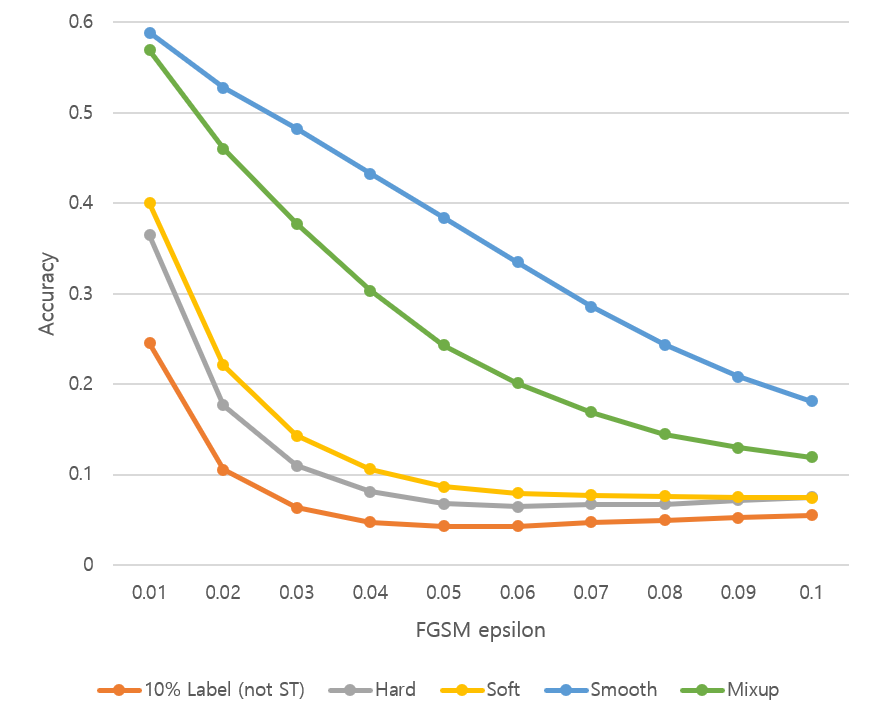
\includegraphics[width=.6\textwidth]{../figz/FGSM}
  \caption{각 pseudo label 타입별 FGSM adversarial attack에 대한 강직도 테스트. 주황색 데이터는 self-training을 거치지 않은 ResNet-38 데이터이다.}
  \label{fgsm}
\end{figure}

위 방식으로 공격 이미지 $\vec x'$를 만들었다. 여기서 $\epsilon$은 공격의 강도로 취급할 수 있으며, 나는 이 공격을 이미지의 각 픽셀 RGB 값을 $[0, 1]$ 범위 값으로 바꾼 상태에서 적용하였다.

그림 \ref{fgsm}에서 같이 초기 teacher model에 비해서 더 높은 강직도를 획득했음을 알 수 있었다. Hard보다는 soft가, 그리고 그것보다 mixup과 label smoothing이 훨씬 좋았다. \cite{goibert2019adversarial}와 \cite{zhang2018mixup}에서 언급했던 두 방법의 강직성이 noisy student 방식에서도 그대로 나타났다.

\subsection{Calibration Errors \& Robustness on Corruptions/Perturbations} Calibration error와 다른 여러 지표들도 분석해보았다. Calibration error란 모델이 예측한 confidence 값과 실제 accuracy가 얼마나 차이가 있는지 확인하는 지표로, 모델의 overconfident 문제를 진단할 수 있다. \cite{guo2017calibration} 보통 ECE(expected calibration error)로 측정한다. Confidence 결과를 $0.1$ 단위로 총 10개의 묶음으로 쪼개어, 각 묶음 별로 실제 accuracy와 confidence의 평균이 얼마나 차이가 나며, 그 차이의 평균을 나타내는 지표이다. ECE 값이 차이가 적게 나야 중요한 의사 결정에서 모델이 말하는 confidence를 신뢰할 수 있을 것이므로 좋은 모델이라고 간주할 수 있다.

또한 CIFAR-10 이미지를 corruption 시킨 CIFAR-10-C 데이터셋과, perturbation 시킨 CIFAR-10-P 데이터셋을 구하여 돌려보기도 하였다. 둘은 \cite{hendrycks2019benchmarking}에서 제안된 데이터로, 실제 이미지 분류 문제에서 자주 직면하는 여러 오염적인 상황들이 적용된 이미지를 테스트하는데 사용한다. 본래 ImageNet-C, ImageNet-P가 더 보편적이지만, 본 프로젝트에서 학습한 데이터가 CIFAR-10이므로, 이를 오염시킨 데이터셋으로 실험하였다.

ImageNet-C에서는 각 오염 요소에 따른 5개의 강도마다 CE(corruption error)를 구하고, 이를 기준 네트워크인 AlexNet과 비교를 통해 relative mCE(mean CE)를 계산하여 오염에 대한 강직성을 수치화시킨다. \cite{hendrycks2019benchmarking}

\begin{align*}
  CE_{c}^f &= \frac{\left( \sum_{s=1}^5 E_{s,c}^f - E_{clean}^f \right)}
  {\left( \sum_{s=1}^5 E_{s,c}^{AlexNet} - E_{clean}^{AlexNet} \right)} \\
  mCE^f &= \frac{1}{|C|} \sum_{c \in C} CE_{c}^f
\end{align*}

또한, ImageNet-P에서는 각 오염 요소마다, 오염 요소의 강도별로 얼마나 많은 예측 결과들이 달라지는지 FP(flip probability)를 통해 강직성을 검사한다. 이 또한 각 perturbation에 대해 기준 네트워크인 AlexNet과 비율을 계산하여 평균을 내는 방식으로 mFP(mean FP)를 계산하여 수치화시킨다. \cite{hendrycks2019benchmarking}

\begin{align*}
  FP_{p}^f &= \frac{1}{m(n-1)} \sum_{i=1}^m \sum_{j=2}^n \vec{1}
  \left( f(x_j^{(i)}) \neq f(x_j^{(1)}) \right) \\
  mFP^f &= \frac{1}{|P|} \sum_{p \in P} \frac{FP_p^f}{FP_p^{AlexNet}}
\end{align*}

문제는 ImageNet에서 AlexNet과 달리 CIFAR-10 문제의 준 지도학습 결과에 대한 기준 네트워크 정보가 없다는 것이다. 그래서 나는 이 프로젝트에서 대조군으로 사용하기 위해 self-training 없이 5,000개의 training data로 학습한 ResNet-38을 기준 네트워크로 설정하여 위 수치들을 계산해보았다.

\begin{table}[!h]
  \center
  \begin{tabular}{ |c|c|c|c|c|c| }
    \hline
      Label Type & Network & Top-1 Acc. & ECE & Rel. mCE & mFR \\ \hline
      Teacher & ResNet-20 & 82.27 & 0.1142 & 117.29 & 105.90 \\ \hline
      Hard & ResNet-26 & 86.36 & 0.0762 & 103.10 & 86.18 \\ 
       & ResNet-32 & 87.58 & 0.0954 & 87.36 & 82.64 \\ 
       & ResNet-38 & 88.28 & 0.0814 & 75.61 & 75.11 \\ \hline
      Soft & ResNet-26 & 86.03 & 0.0494 & 77.16 & 85.51 \\
       & ResNet-32 & 87.68 & 0.0355 & 56.54 & 77.60 \\ 
       & ResNet-38 & 88.21 & 0.0495 & 72.95 & 70.16 \\ \hline
      Smooth & ResNet-26 & 86.19 & 0.0328 & 66.30 & 81.52 \\
       & ResNet-32 & 87.73 & 0.0504 & 74.72 & 78.07 \\ 
       & ResNet-38 & 88.48 & 0.0789 & 76.94 & 73.39 \\ \hline
      Mixup & ResNet-26 & 86.34 & 0.1056 & 60.31 & 83.91 \\
       & ResNet-32 & 86.70 & 0.0263 & 68.51 & 80.07 \\ 
       & ResNet-38 & 87.78 & 0.0780 & 50.11 & 75.58 \\ \hline
      Without ST & ResNet-38 & 83.91 & 0.1169 & 100.00 & 100.00 \\ \hline
  \end{tabular}    
  \caption{각 pseudo label 타입별 calibration error 및 corruption/perturbation robustness 지표. Top-1 accuracy 외 모두 낮은 수치가 좋다.}
  \label{robustness}
\end{table}

표 \ref{robustness}와 같이 결과가 나타났다. 우선 calibration error의 경우 모두 마지막 네트워크에서 ECE $0.1$ 이내의 준수한 값이 나타났으며, soft label에서 가장 적었다. 반면 overconfident 문제를 초래할 것으로 예측되었던 hard label에서 가장 높게 나타났지만, 여전히 원래 방식보다 적은 수치였다. Relative mCE의 경우 hard, soft, smooth label에서는 비슷한 값이 나타났지만, mixup 방식에서 압도적으로 높은 성능이 보였다. 하지만 mFR의 경우 soft가 미세한 차이로 좋았지만, 여러 모델 간의 큰 차이는 도드라지지 않았다. 이를 통해 soft label, mixup 방식이 비교적 적은 수의 pseudo label 정보를 받았다는 점에서 top-1 accuracy를 내는 것에는 불리했지만, 더 overconfident 문제에서 자유로우며, 강직성이 높은 모델을 학습했음을 추론할 수 있었다.